\documentclass[tikz,border=2pt]{standalone}
\usepackage{amsmath,amssymb}
\usepackage{pgfplots}
\pgfplotsset{compat=1.18}
\usetikzlibrary{arrows.meta}
\begin{document}
% Erlang B blocking probability B(c,3) for c = 1..10 (offered load a = lambda/mu = 3), log scale:
% 0.75, 0.529, 0.346, 0.206, 0.110, 0.0522, 0.0219, 0.0081, 0.0027, 0.0008; target 1%: first c is 8.
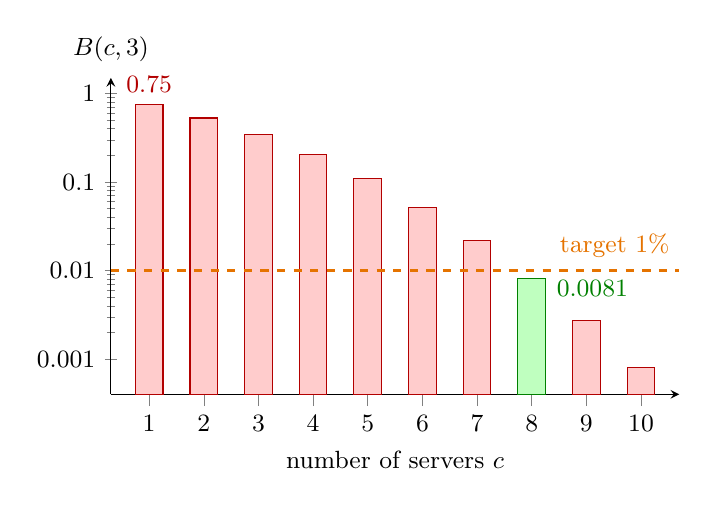
\begin{tikzpicture}[font=\small, >={Latex[length=2mm]}]
  \begin{axis}[
    axis lines=left, ymode=log, ymin=0.0004, ymax=1.5, xmin=0.3, xmax=10.7,
    xtick={1,...,10}, ytick={0.001,0.01,0.1,1}, yticklabels={$0.001$,$0.01$,$0.1$,$1$},
    ybar, bar width=10pt, bar shift=0pt, log origin=infty,
    xlabel={number of servers $c$}, ylabel={$B(c,3)$},
    ylabel style={rotate=-90, anchor=south, at={(axis description cs:0,1.02)}},
    width=8.8cm, height=5.6cm, clip=false]
    \addplot[draw=red!70!black, fill=red!20] coordinates {(1,0.75) (2,0.52941) (3,0.34615) (4,0.20611) (5,0.11005) (6,0.05216) (7,0.02186) (9,0.0027) (10,0.00081)};
    \addplot[draw=green!50!black, fill=green!25] coordinates {(8,0.00813)};
    \draw[orange!90!black, thick, dashed] (axis cs:0.3,0.01) -- (axis cs:10.7,0.01);
    \node[orange!90!black, anchor=south east] at (axis cs:10.7,0.011) {target $1\%$};
    \node[green!50!black, anchor=west] at (axis cs:8.28,0.0062) {$0.0081$};
    \node[red!70!black, anchor=south] at (axis cs:1,0.8) {$0.75$};
  \end{axis}
\end{tikzpicture}
\end{document}
